\chapter{Experiments and observations}
\label{ch:experiments}

Based on our own experience and anecdotal evidence, we have set goals and priorities during the development of Sensei.
During my research, I conducted various experiments and interviews to asses these priorities, and to evaluate the various features as described in the previous chapter.
In this chapter, I describe the goal of each experiment, its set-up, and report the findings.

\summarybox{
I conducted a controlled user experiment that showed Sensei markings are easy to understand and quick-fixes are applied frequently.
Addressing security problems like this with Sensei, only caused an average increase in development time of about 11\%.

Interviews with security professionals showed that the tool can be used effectively in a professional setting to detect and remediate security problems.
They describe the customization of recipes as being easier and faster compared to other security tools.
Nonetheless, usability experiments showed that the \gls{yaml} code used for recipes can be overwhelming and that all users prefer the \gls{ui} view of the new recipe editor.
Creating new recipes was more successful if the users followed along with documentation, or if they looked at example recipes first, creating recipes from scratch can still be difficult.

The biggest disadvantages of Sensei compared to other tools are its lack of reported metrics and its poor integration in the \gls{cicd} pipeline.
}

%\todo[inline]{compare results to those of rasch model}

\section{Controlled empirical usability experiment}
\label{sec:experiment}

In November 2018, I conducted an experiment with students to evaluate some features of the Sensei \gls{ide} plugin.
This experiment has been well designed with the help of my supervisors and prof. Riccardo Scandariato who has practical experience with similar experiments.
It was conducted with the help of the lecturer, dr.\ ir.\ Mattias De Wael, and two of my colleagues at \gls{scw}, Downey Robersscheuten and Tim Dekiere.
%Due to complications during the hand-in procedure, the results of this experiment are mostly focused on the usability of the tool.
%We are able to make observations regarding the amount of violations that are resolved and how fast they are resolved.
%However, we cannot make any claims on the resulting security implications.

\subsection{Goals and research questions}
The main \textit{goal} of the experiment is to observe the impact of the Sensei \gls{ide} plugin on developers and their code.
The \textit{purpose} is evaluating the usability and effectiveness of several of the features offered by Sensei during development, such as customized guidelines and quick-fixes in the \gls{ide}.
The \textit{quality focus} is the ability of the plugin to help developers adhere to secure coding guidelines without causing a significant cognitive burden.
The study evaluates the behaviour of a developer.
We aim at measuring the increase in cognitive burden when developers use the plugin, by measuring the impact on development time.
In our experiment, we evaluated the impact on a group of students who have a consolidated minimum level of expertise in both web application development and web application security.

The above goal can be achieved by means of an experiment aimed at answering the following four questions:
\begin{itemize}
    \item \textbf{Q1} How effective are the Sensei code markings at grabbing the developer's attention?
    \item \textbf{Q2} Does the plugin significantly impact the development time?
    \item \textbf{Q3} Do developers often use the provided remediation (quick-fixes) to resolve code markings?
    \item \textbf{Q4} Are there any specific code markings that significantly impact the usability compared to others?
\end{itemize}

\subsection{Experimental set-up}
\subsubsection{Subjects}
The subjects for this study are a group of third year students following the bachelor program for Computer and Cyber Crime Professional\footnote{\url{https://www.howest.be/en/study-programmes?s_filter=bachelor}} at the college Hogeschool West-Vlaanderen (Howest) in Bruges, Belgium.
All students are in the third, and final year of the bachelor program.
The experiment was performed in the context of the Secure Object Oriented Architectures class.
In this course, the students are taught design patterns, how to design three-layered applications, and Java technicalities.
During the entire course the focus is on development while conforming to Oracle's Secure Coding Guidelines\footnote{\url{https://docs.oracle.com/cd/E26502\_01/html/E29016/scode-1.html}}.

All of the students are familiar with Java programming in IntelliJ IDEA, as it is the main language and \gls{ide} used in the education program.
They are, however, not experienced or trained with the Sensei tool.
This experiment was their first exposure to the tool. 

The experiment was preceded by a secure coding tournament using the \gls{scw} platform.
The goal of this tournament was to both engage the students as well as measure their skill level.
Student participation was voluntary, out of the 75 students that participated in the tournament, 60 also participated in the experiment itself.
However, only 32 students successfully submitted all necessary files after the experiment, as will be described further down this section.

\subsubsection{Development task}
\label{sec:task}
The subjects were given a development task to complete with the Sensei plugin installed in their \gls{ide}.
For the assignment they received the incomplete code for an employment web app.
The application provides employees of a company a way to view, download, and upload their payslips, as well as to submit requests for absence.
The application is written in Java and uses \gls{jsp} as the server side technology.
Some of the features are incomplete and must be completed by the subjects during the experiment.
During the implementation of these features, the subjects are at risk of introducing a number of web application vulnerabilities.
Below is a list of features to be completed and their associated risks.

\begin{itemize}[noitemsep]
    \item A web page to view absence requests: risk of \gls{xss}.
    \item A web form to search for absence requests in the database: risk of \gls{sql} injection.
    \item A web form to upload payslips in \gls{xml} format: risk of \gls{xml} injection, \gls{xml} external entity, unrestricted file upload, and local file inclusion.
    \item Log all attempts made on the sign-in page: risk of log forgery.
\end{itemize}

\subsubsection{Treatment}
The treatment consisted of two parts. First, all subjects participated in a \gls{scw} tournament.
The next week, all participants were given the Sensei \gls{ide} plugin, but some features were disabled for the control group.
\paragraph{Tournament}
One week preceding the experiment, all subjects participated in a tournament on the \gls{scw} platform.
The subjects were handed 24 secure coding exercises in Java using \gls{jsp} to complete within 90 minutes.
The awarded points on completion of an exercise depends on its difficulty and the performance of the subject, as described in Appendix~\ref{app:challenges}.
The scoring method chosen was ``Forgiving".

The total maximum score for all exercises in the tournament was 5000 points.
The highest score reached was 4920, while the lowest was 1600.
The mean score reached by the participants (n = 75) was 3659 (s = 710).
The mean time spent solving all exercises was 53.70 min (s = 16.07 min).
Both the score and the time spent are approximately normal distributions as shown in Figure~\ref{fig:hist-score} and Figure~\ref{fig:hist-time}.
The score reached by each subject in this tournament was used to split the subjects into two equally skilled groups, a control group and a test group.
The subjects were told that they were participating in an experiment regarding the Sensei plugin.
They were told that they were split in a control group and test group but were not informed of which group they were part, or what the difference in treatment would be. 

\begin{figure}
    \centering
    %\begin{tikzpicture}
    \node at (0,0) {
        \begin{tikzpicture}
        \begin{axis}[
            %ybar interval,
            ymax=24, ymin=0,
            xmin=1500, xmax=5000,
            xtick = {1500,5000},
            xtick pos=bottom,
            grid=none,
            ytick pos=left,
            ytick = {-1,25},
            y axis line style={draw=none},
            x axis line style={color=gray},
            x tick label style={color=gray,
                yshift={-1em},
                /pgf/number format/.cd,fixed,precision=3, set thousands separator={}},
            y tick label style={color=gray},
            ]
            
            \addplot [
            scw-teal,
            fill=scw-teal,
            ybar interval,
            mark=none,
            ]
            coordinates
            {
            (1500, 2)
            (2000, 1)
            (2500, 10)
            (3000, 14)
            (3500, 24)
            (4000, 14)
            (4500, 9)
            (5000, 0)
            };
    
        \end{axis}
        \end{tikzpicture}
    };
    
    %x axis
    \node[gray] at (0.9,-3.05) {3659 points};
    \draw[thick, lightgray] (-3.47,-2.7) -- (3.42,-2.7);
    \draw[thick, lightgray] (-3.47,-2.7) -- (-3.47,-2.6);
    \draw[thick, lightgray] (3.42,-2.7) -- (3.42,-2.6);
    \draw[thick, lightgray] (0.9,-2.7) -- (0.9,-2.6);
    
\end{tikzpicture}
  \includegraphics[page=17]{03-education/figures/tikzfigures.pdf}
  \caption[Histogram of points scored in the \gls{scw} tournament]{The points scored by the subjects during the tournament is approximately a normal distribution around the mean of 3659 points.}
  \label{fig:hist-score} 
\end{figure}

\begin{figure}
    \centering
  % \begin{tikzpicture}
    \node at (0,0) {
        \begin{tikzpicture}
        \begin{axis}[
            %ybar interval,
            ymax=17, ymin=0,
            xmin=10, xmax=100,
            xtick = {10,100},
            xtick pos=bottom,
            grid=none,
            ytick pos=left,
            ytick = {-1,20},
            y axis line style={draw=none},
            x axis line style={color=gray},
            x tick label style={color=gray, yshift={-1em}},
            y tick label style={color=gray},
            ]
            
            \addplot [
            scw-teal,
            fill=scw-teal,
            ybar interval,
            mark=none,
            ]
            coordinates
            {
            (10, 1)
            (20, 4)
            (30, 11)
            (40, 17)
            (50, 15)
            (60, 15)
            (70, 9)
            (80, 2)
            (90, 1)
            (100, 0)
            };
    
        \end{axis}
        \end{tikzpicture}
    };
    
    %x axis
    \node[gray] at (0,-3.05) {54 min};
    \draw[thick, lightgray] (-3.47,-2.7) -- (3.42,-2.7);
    \draw[thick, lightgray] (-3.47,-2.7) -- (-3.47,-2.6);
    \draw[thick, lightgray] (3.42,-2.7) -- (3.42,-2.6);
    \draw[thick, lightgray] (0,-2.7) -- (0,-2.6);
    
\end{tikzpicture}
  \includegraphics[page=18]{03-education/figures/tikzfigures.pdf}
  \caption[Histogram of time spent in the \gls{scw} tournament]{The time spent by the subjects (n=75) competing in the tournament is approximately a normal distribution around the mean of 54 min.}
  \label{fig:hist-time} 
\end{figure}


\paragraph{Sensei}
To complete the programming exercise, the subjects on both groups were allowed to use their own device and \gls{os} but they had to develop using the IntelliJ IDEA with the Sensei plugin installed.
The Sensei installation of both the control group and the test group included a set of carefully tailored recipes to prevent introduction of the vulnerabilities described in Section~\ref{sec:task}.
However, for the control group the markings and programming aid were disabled and the plugin was only used as a monitoring tool.
All features to view, edit, or disable recipes were hidden, so that none of the subjects were able to consult or alter the recipes.
The information available to the subjects, in the different descriptions, was designed as outlined in Section~\ref{sec:information}.
In fact, the example given in Figure~\ref{fig:fulldescription} is a guideline used during the experiment.

\subsubsection{Ethical review board}
The teaching staff proposed the experiment to the college's ethical review board.
We helped them in writing a detailed explanation of the activities and the goals of the experiment.
The board approved the experiment under two conditions.
Firstly, experiment participation was to be voluntary and students were not to receive extra credit upon participation.
Secondly, all data handed to the researchers was to be made completely anonymous.
We and the teaching staff then operated in line with these conditions.

\subsubsection{Experimental procedure}
The experimental procedure is split into two main activities, the controlled experiment itself and the post-experimental information gathering.

\paragraph{Controlled experiment}
All subjects were allowed to use their own devices, and any resources they would normally use during development, such as books and internet access.
We did not allow communication with other subjects.
Subjects were allowed to take breaks and leave the room.
However, as to not give incentive to finish hastily and without care, all subjects were required to be present during debriefing.
The subjects installed Sensei by adding a custom repository instead of through the JetBrains Marketplace, as this allowed us to customize the features of the plugin for this experiment.

The subjects were given:
\begin{itemize}[noitemsep]
    \item a consent form to acknowledge that their data will be analysed anonymously;
    \item a repository \gls{url} to install the Sensei plugin, which automatically includes the set of recipes for each subject;
    \item a link to an archive containing the \gls{ide} project for the assignment;
    \item plugin installation instructions;
    \item a detailed description of the programming assignment.
\end{itemize}

During the controlled experiment, we asked the subjects to complete the assignment using the procedure below.

\begin{enumerate}[noitemsep]
    \item Open the plugins menu in the \gls{ide} and copy-paste the \gls{url} to the plugin repository.
    \item Install the plugin and restart the \gls{ide} after the process has completed.
    \item Verify correct installation of the plugin by finding the ``Sensei" menu in the menu bar of the \gls{ide}.
    \item Download the archive containing \gls{ide} project.
    \item Extract the archive and open the project in the \gls{ide}.
    \item Execute the project and read the messages in the console.
    \item Open a web browser and browse to \texttt{localhost} to verify that the project is running correctly.
    \item Sign in using provided credentials and get familiar with the functionality of the web application.
    \item Read the description of the features to be implemented.
    \item Complete the programming assignment in silence.
\end{enumerate}

Throughout all phases of the experiment, we provided assistance to the subjects and answered all questions unrelated to the security of their code or the information displayed by the plugin.
Indeed, despite testing on several operating systems and \gls{ide} versions there were some setup issues to solve.

\paragraph{Post-experiment information gathering}
\label{sec:after}
When the task had been completed or the allocated time ended, the subjects were instructed to:

\begin{enumerate}[noitemsep]
    \item navigate to the Sensei installation folder and find the Sensei events file, which contains a log of all the actions monitored by the Sensei plugin
    \item archive both the events file and the source files into one archive
    \item submit the archive to the teaching staff
\end{enumerate}

The events file contains timestamps and guidelines for all logged events.
Examples of event files are shown in Table~\ref{tab:recipe1}, and Table~\ref{tab:recipe2}.
The events in these tables include newly introduced guideline violations (ADD) that are later in time removed (DELETE).
In Table~\ref{tab:recipe2} violations are removed using quick fixes (FIX).
The removal of a guideline violation leads to compliant code.
Sometimes it is possible to detect this compliant code with a different Sensei recipe that is marked as a compliant counterpart (C\_ADD).
For example, a parameterized query is the compliant counterpart of a \gls{sql} injection.
A compliant counterpart is available for the recipe in Table~\ref{tab:recipe1}.
For other recipes, such as the one in Table~\ref{tab:recipe2}, no compliant counterpart can be created.
This is not possible, for example, for a recipe that forbids the use of \gls{os} commands, in order to prevent \gls{os} command injection.
All code devoid of \gls{os} commands is technically compliant to this recipe, but we cannot create a recipe that detects conscious compliance to the recipe.
The events also include the opening of a description (DESCRIPTION).
The events file does not include code or code locations, as our clients do not want to expose this information.

\begin{table}
    \centering
    \begin{tabular}{|l|}
      \hline
      \cellcolor{scw-orange!30}
      ADD\\
      \cellcolor{scw-teal!30}
      DELETE\\
      C\_ADD\\
      \cellcolor{scw-orange!30}
      ADD\\
      DESCRIPTION\\
      \cellcolor{scw-teal!30}
      DELETE\\
      C\_ADD\\
      \hline
    \end{tabular}
    \caption[Sensei events file]{The Sensei events file lists all events chronologically. In this example, a recipe was violated twice (ADD). Both times the violation was subsequently removed (DELETED) and replaced by compliant piece of code (C\_ADD). Before correcting the second violation, the description was opened (DESCRIPTION).}
    \label{tab:recipe1}
\end{table}

%\begin{table}
%\centering
% \begin{tabular}{|l l|} 
% \hline
% Event type & recipe ID \\ 
% \hline
% \cellcolor{scw-orange!30}
% ADD & requestparam \\
% \cellcolor{scw-teal!30}
% DELETE & requestparam \\
% %\cellcolor{apple-green!30}
% C\_ADD & requestparam \\
% \cellcolor{scw-orange!30}
% ADD & requestparam \\
% %\cellcolor{scw-yellow!30}
% DESCRIPTION & requestparam \\
% \cellcolor{scw-teal!30}
% DELETE & requestparam \\
% %\cellcolor{apple-green!30}
% C\_ADD & requestparam \\
% \cellcolor{scw-orange!30}
% ADD & xss \\
% \cellcolor{scw-orange!30}
% ADD & xss \\
% %\cellcolor{scw-teal!30}
% FIX & xss \\
% \cellcolor{scw-teal!30}
% DELETE & xss \\
% %\cellcolor{scw-teal!30}
% FIX & xss \\
% \cellcolor{scw-teal!30}
% DELETE & xss \\
% %\cellcolor{apple-green!30}
% C\_ADD & sqlinjection \\
% \hline
%\end{tabular}
%\caption[Example of a Sensei events file]{The Sensei events file lists all events chronologically. In this example, the requestparameter recipe was violated twice (ADD). Both times the violation was subsequently removed (DELETED) and replaced by compliant piece of code (C\_ADD). Before correcting the second violation, the description was opened (DESCRIPTION). The xss recipe was first violated twice and then both instances were fixed using the quickfixes (FIX), no compliant counterpart exists for the xss recipe. From this information it is impossible to assert which of the xss recipe violations was removed first. The sqlinjection recipe was never violated, but a compliant piece of code has been added.}
%\label{table:events}
%\end{table}

Several days after the experiment, all data was handed to us by the teaching staff after having obscured all personal data.
At this point we discovered that the hand-in procedure was not correctly performed by all subjects, as the majority of the subjects had handed in either the code or the events file but few handed in both as requested.
We asked all subjects to hand in again, stressing to include both the events file and all source files, but few subjects submitted a second time. 

Without the source code in addition to the events file, I am unable to verify whether the code is still functional, as simply removing the relevant pieces of code would also effectively remove all guideline violations.
On the other hand, without the events file we cannot verify which impact the Sensei plugin had on the security of resulting code.

This means I do not have sufficient data to compare results from both groups to evaluate the \textit{effectiveness} of Sensei on improving the security of the final code, but that was never the main objective of the experiment.
%It remains future work to rerun a similar experiment including the proper collection of all required data.
With the data from the 32 subjects who handed in their events file, I can still evaluate the \textit{usability} of Sensei, albeit with a smaller data set than intended.

\subsubsection{Analysis method}
\label{sec:analysis}
Since the logs in the events file do not include file locations, we sometimes have to make assumptions on which ADD and DELETE events should be paired.
On occasion, there are multiple guideline violations with the same recipe ID present in the code at a certain time, as is the case in Table~\ref{tab:recipe2}. 
In this case, we cannot know for certain which of the two violations is fixed first.
During our experiment, this was the case for 8\% guideline violations, with the two ADD events on average 37.75 s (s = 44.05 s) apart.
For the measurements of the time between adding the violation and removing it, we assumed that the violations were removed in the same order as they were introduced.
For all of the cases eventually either both violations were removed or neither of them were.
The aforementioned assumption hence has no influence on the mean removal time and only influences the standard deviation of the removal time. 

\begin{table}
    \centering
    \begin{tabular}{|l|}
      \hline
      \cellcolor{scw-orange!30}
      ADD \\
      \cellcolor{scw-orange!30}
      ADD \\
      FIX \\
      \cellcolor{scw-teal!30}
      DELETE \\
      FIX \\
      \cellcolor{scw-teal!30}
      DELETE \\
      \hline
    \end{tabular}
    \caption[Sensei events file with multiple violations at the same time]{In this Sensei events file the recipe was first violated twice and then both instances were fixed using the quick fixes (FIX), no compliant counterpart exists for this recipe. From this information it is impossible to assert which of the recipe violations was removed first.}
    \label{tab:recipe2}
\end{table}

We observed three exceptionally long removal times and inspected the logs to determine the cause.
Two of the outliers had events regarding other recipe IDs in between the ADD and DELETE events and so the subject did not spend this time actively solving the guideline violation.
For further computations of removal time, these two outliers are left out.
In between the ADD and DELETE events of the third case there were a number of DESCRIPTION events with the same recipe ID. In this case, we can safely assume that the subject did indeed spend 3.54 min actively resolving the issue.

\subsection{Findings}
\subsubsection{Guideline violations}
On average, the subjects in the test group introduced 17.64 guideline violations, as shown in the top right of Figure~\ref{fig:hist-control-test}.
The best performing subject (in this regard) introduced 2 guideline violations.
For this subject, the events log showed enough C\_ADD events to assume that the subject completed at least the majority of the programming exercise.
The worst performing subject added 37 guideline violations.
In this case the events log showed a large number of ADD and DELETE events for the same recipe ID, making us believe that the subject was rewriting the code a number of times.
This can result from attempting to implement the code functionally correctly or from attempting to resolve the guideline violation.
The absence of DESCRIPTION events in the log is strong evidence for the former. 

In the control group the average number of violations introduced is 24.7, as shown in the bottom left of Figure~\ref{fig:hist-control-test}.
The amount of violations introduced in this group is between 2 and 54, however this distribution is not statistically significantly different from the test group as determined by a Games-Howell post-hoc test (p = 0.11).

After completion of the assignment, the test group had 0.22 remaining guidelines on average, as shown in the top right in Figure~\ref{fig:hist-control-test}.
Out of these subjects, 79\% (n = 12) finished the assignment free of violations.
The average number of violations left at the end of the assignment in the control group was 8.8 and only 6\% (n = 1) of the subjects finished the assignment without any remaining violations.
This is shown in Figure~\ref{fig:hist-control-test} in the bottom right.
This difference in remaining violations between the two groups is statistically significant (p = 0.00015).

\begin{figure}
  \begin{subfigure}[t]{.49\textwidth}
    \centering
     \includegraphics[page=24,width=\linewidth]{03-education/figures/tikzfigures.pdf}
  %\caption[Histogram of violations added by the test group]{The amount of violations added by each subject in the test group is between 2 and 37. On average 17.6 violations have been added.}
  %\label{fig:hist-added-test} 
  \end{subfigure}
  \hfill
    \begin{subfigure}[t]{.49\textwidth}
    \centering
   \includegraphics[page=26,width=\linewidth]{03-education/figures/tikzfigures.pdf}
  %\caption[Histogram of violations left by the test group]{left test}
  %\label{fig:hist-left-test} 
  \end{subfigure}
  
  \begin{subfigure}[t]{.49\textwidth}
    \centering
    \includegraphics[page=25,width=\linewidth]{03-education/figures/tikzfigures.pdf}
  %\caption[Histogram of violations added by the control group]{The amount of violations added by each subject in the control group lays between 2 and 54. On average 24.7 violations have been added.}
  %\label{fig:hist-added-control} 
  \end{subfigure}
  \hfill
  \begin{subfigure}[t]{.49\textwidth}
    \centering
   \includegraphics[page=27,width=\linewidth]{03-education/figures/tikzfigures.pdf}
  %\caption[Histogram of violations left by the control group]{left control}
  %\label{fig:hist-left-control} 
  \end{subfigure}
  
  \caption[]{Histograms of the amount of violations introduced during the assignment (left column) and remaining at the end of the assignment (right column) by users in the test group (in orange) and the control group (in blue). The amount of violations introduced by the two groups is not statistically significantly different. The amount of violations left at the end of the assignment is significantly more for the control group.}
  \label{fig:hist-control-test}
\end{figure}

\subsubsection{Resolving guideline violations}
Out of all the coding guideline violations in the test group, 98.4\% have been removed eventually.
Out of the removed violations, 73.3\% have been removed with a quick-fix.
For the remaining removals, it is not possible to know the intention of the subject, i.e., whether the violations were resolved manually as the subject spotted them as violations or whether the removal was part of rewriting (or removing) the code for another reason, such as simply meeting the functional requirements of the assignment.
The four unresolved guideline violations each violated one different guideline, so there was no particular guideline causing the majority of usability problems.
One was violating a \gls{sql} query guideline and the others were violations of several file upload guidelines by the same user.

Out of the violations that were resolved, 89.3\% were resolved within one minute, and 99.5\% were resolved within three minutes.
Only one case, previously discussed in Section~\ref{sec:analysis}, took 3.54 min to resolve.
This subject did eventually not use the quick-fix to resolve the issue.
There is no pattern in the guidelines of the 10.7 \% of violations that were not resolved within 1 minute.
These violations are distributed evenly over the 7 guidelines that have the longest mean remediation time.

On average the subjects of the test group took 19.10 s (s = 25.22 s) to resolve an issue.
This large standard deviation is explained by a large difference in removal time for certain guidelines, as can be seen in Figure~\ref{fig:fixtimes}.
The mean remedation time when a quick-fix was used was 17.36 s.
The violations that were removed by the subjects of the test group without a quick-fix were resolved in 21.73 s on average.
The influence of the quick-fix on the remediation time is not statistically significant (p = 0.7).
The average remediation time in the control group was 129.21 s (s = 422.26 s), and this is significantly different from the remedation time in the test group (p = 0.001).

On average more commonly known vulnerabilities such as \gls{sql} injection and \gls{xss} are resolved within less than 10 seconds, while the guidelines regarding file upload vulnerabilities take significantly longer.
This is in line with general results from the trained \gls{2pl} model in the experiment of Section~\ref{sec:eval-rasch}.
The model showed that exercises about commonly known vulnerabilities such as \gls{sql} injection and \gls{xss} have a lower mean difficulty on the \gls{scw} training platform.
Both these results indicate that understanding and fixing these common vulnerabilities is relatively easy.
But in this experiment, as well as in practice, many developers still make those mistakes.
This gap between knowledge and practice shows that when developers are focused on the functionality of their code, they can easily lose track of the security.

Besides familiarity with the vulnerability, the difference in speed for resolving the vulnerabilities can also be explained by the fact that one piece of code can violate multiple guidelines.
This was often the case for the file upload guidelines, the naive implementation without any security checks violates guidelines regarding file path, file size, and file extension.
The developers violating these guidelines receive a lot of simultaneous feedback, which takes longer to process.
Fixing these vulnerabilities then also involves slightly larger pieces of code, as opposed to the often single line of code that needs to be fixed for the other guidelines.
This is also in line with observations of the \gls{2pl} model, where the locality of the fix has a big influence on the mean difficulty of exercises.

\begin{figure}
  \centering
  %\begin{tikzpicture}

    %\draw [ultra thin, scw-teal] (1.45,3.5) -- (1.45,-3.5);
    
    \node at (0,0) {
        \begin{tikzpicture}
          \begin{axis}[
            xbar,
            y axis line style={ opacity=0 },
            axis x line=none,
            y tick label style={
                color=gray,
                align=left
                },
            tickwidth=0pt,
            xmin=0,
            xmax=38,
            y=20pt,
            ytick=data,
            nodes near coords,
            nodes near coords style={
                color=gray
            },
            visualization depends on={x \as \myx},
            every node near coord/.append style = {
                shift = { (axis direction cs: 39-\myx,0) }     
            },
            yticklabels = {
                {SQL    },
                XSS,
                {Input validation (2)},
                Stacktrace printing,
                {Input validation (1)},
                Information leakage,
                Log forgery,
                File path,
                File extension,
                File size
            },
            ymajorgrids={true},
            ]
            
            \addplot 
            [scw-teal,
            fill=scw-teal]
            coordinates
            {
            %(4,{SQL})
            %(7,XSS)
            %(15,{Input validation (2)})
            %(21,Stacktrace printing)
            %(27,{Input validation (1)})
            %(29,Information leakage)
            %(30,Log forgery)
            %(32,File path)
            %(35,File extension)
            %(38,File size)
            (4,1)
            (7,2)
            (15,3)
            (21,4)
            (27,5)
            (29,6)
            (30,7)
            (32,8)
            (35,9)
            (38,10)
            };
            
          \end{axis}
        \end{tikzpicture}
    };
    
    \node [left,gray] at (5.6,3.8) {mean removal time [s]};
    
    \node [left,gray] at (-2.05,-3.8) {overall mean};
    
    %\node [scw-teal] at (1.45,-3.8) {overall mean};
    %\node [right,scw-teal] at (5,-3.8) {19};
    
    % circle on a line
    %\draw [ultra thin, lightgray] (-2,-3.8) -- (4.85,-3.8);
    %\node at (1.45,-3.8) [circle,fill,inner sep=1.5pt,scw-teal]{};
   
    % rectangle with a line 
    \draw [ultra thin, lightgray] (1.45,-3.8) -- (4.85,-3.8);
    \draw[scw-teal](-2,-3.6) rectangle (1.45,-4);
    \node [right,gray] at (5,-3.8) {19};

    
\end{tikzpicture}
  \includegraphics[page=19]{03-education/figures/tikzfigures.pdf}
  \caption[Average removal time of guidelines]{The average removal time for each guideline fluctuates heavily and many are different from the overall mean removal time of 19.10 seconds.}
  \label{fig:fixtimes}
\end{figure}

All of the subjects used at least one quick-fix, with an average of 12.71 (s = 4.73) quick-fixes used per subject.
Less than half of the users (42.85\%) have opened a description.
On average the subjects opened 2.79 (s = 7.64) descriptions.

\subsubsection{Development time}
Using the events file from Sensei we can determine the approximate development time for the entire experiment.
If we take the time difference between the first and the last event, this will likely be close to the total development time.
This can be done for all users of both the control and the test group that handed in the events file.
For users in the test group we can also approximate the time spent addressing Sensei markings by taking the sum of all removal times.
We can compare these results to see how much impact Sensei had on the development time.
Users of the control group (n = 17) spent on average 61.54 min (s = 17.68 min) to complete the experiment.
Users of the test group (n = 15) spent on average 68.75 min (s = 14.42 min).
This is an increase of 11.72\% in development time when using the plugin.
The time spent by the test group addressing coding guideline violations was on average 8.42 min (s = 10.06 min).
The average share of total development time that is spent addressing guideline violations is 11.28\% (s = 12.25\%).
This is consistent with the previously measured 11.72\% increase in development time.

\subsection{Threats to validity}
In this section, I check the experiment against the possible threats to validity as proposed by Wohlin et al.~\cite{wohlin2012experimentation}. 

\subsubsection{Conclusion validity}% threats. These are issues that affect the ability to draw the correct conclusion about relations between the treatment and the outcome of the experiment.
The final score of each subject in the tournament is not a complete estimate of the subject's skills regarding security or secure development.
Since there is a time limit, a good score is also partly achieved by time management.
On one hand, taking too much time to complete the exercises will result in missed scoring opportunities by not finishing all exercises.
On the other hand, answering too hastily may result in mistakes that otherwise could have been avoided, again resulting in a loss of points.
However, the exercises were in the same language and framework as the development task, and the subjects also had a limited time to complete this task, so it is a reasonable estimate.
 
Each group of subjects were given the exact same development exercise, only different treatment.
 
The subjects were not heterogeneous, as they were all bachelor students, and the tournament score was used to avoid random irrelevance to some degree.

\subsubsection{Internal validity}% are influences that threat the conclusion about a possible causal relationship between the treatment and the outcome. Here we discuss all sources of noise and discuss how they have been either eliminated or measured.
Before starting the experiment, we clearly explained the programming assignment and answered any arising questions publicly.
The experiment itself was conducted in a single session, with all participants in the same room, this excludes all threats related to location, and repetitions.

Since the experiment was preceded by a secure coding tournament, and the experiment took place in a security oriented class, this history can affect the experimental results.
However, do note that the entire bachelor's program followed by the subjects is focused on security, so the security related activities are not that different from usual day-to-day activities.

Since the experiment took over an hour, depending on the speed of development, subjects may react differently as time passes.
Indeed, to avoid students getting tired, bored, or frustrated, we allowed them to take breaks and leave the room.
We also note that the opposite is possible, and even likely, the subjects could have been learning and adjusting their behaviour during the experiment.
This will also interact with the selection, since the test group receives feedback on their behaviour through the tool, and the control group does not.

The effect of letting volunteers take part in an experiment may influence the result, since they are generally more motivated and suited for a new task than the whole population.
The subjects group might not be representative of the whole population.

Since some of the subjects did not hand in their Sensei events file, it can be useful to characterize the dropouts in order to check if they are representative of the total sample.
However, due to the anonymity of the data, we were unable to do this.

The subjects in the control group are receiving less desirable treatments.
As the natural underdog, they might be motivated to reduce or reverse the expected outcome of the experiment.
This threatens the comparison in development time between both groups.
This effect is expected to be more present if we had been comparing the security of the resulting code, but we did not do this.
Moreover, we took the necessary precautions to avoid that the control group was aware of being in a less desirable situation, such as leaving them unaware of what the Sensei tool looks like, thus leaving them unaware of it being disabled for them.

\subsubsection{Construct validity}% question the relation between the theoretical constructs and the actually metrics in the experiment.
We collected information about the time spent resolving issues as the time between introducing the violation and removing it.
However, during this time window the subjects might still be working on the functionality of the code instead of its security.
Since these two tasks are mostly interleaved, it would be nearly impossible to precisely asses the two times separately.
Hence our focus on the increase in total development time as an additional measurement.

The subjects were aware that they were participating in an experiment.
This in itself may make the subjects more receptive to its feedback.

The subjects were allowed to use any resource they desired to complete the task.
This factor may influence the results, because better resources could help in completing the programming task faster or with less security issues.

The subjects might try to figure out what the purpose and intended result of the experiment is.
They are likely to change their behaviour based on their guesses about the hypotheses.
For this reason we did not disclose to the participants whether or not they were part of the control group or the test group.
But it is likely at least the control group would realise their role in the experiment after not receiving feedback from the tool for a while.
This does not influence our results about the interaction with the tool since the control group does not interact with it.
The test group is less likely to realise their role in the experiment, but the realization is more likely to cause an effect.

Some people are afraid of being evaluated.
A form of human tendency is to try to look better when being evaluated, this could influence how the test group interacts with the tool.
It is possible that the subjects would ignore markings more often if they were not being evaluated.

\subsubsection{External validity}% are conditions that limit our ability to generalize the results of our experiment to industrial practice.
All students come from the same college and the same bachelor's program.
It is possible that subjects from a different college or program might result in different performance while completing the development task.

The subjects were not trained or experienced in the use of the treatment.
It is possible that developers with more experience with security tools in general, or specifically Sensei, behave differently when interacting with the tool.

Since all subjects were tasked to develop a web application using Java JSP, the findings might not relate to development in general.
The findings might not apply to development of other types of software, or when using other languages, or frameworks. 

The subjects mostly lack professional experience, most of them only having done internships.
It is possible that developers with more professional development experience behave differently.
\section{User testing with individual developers}
\label{sec:user-testing}
During my research of the Sensei \gls{ide} plugin, Sensei's product manager at \gls{scw}, Charlie Eriksen, has organized two usability tests.
The first usability test was performed in October 2020, the second several months later in April 2021.
The usability tests were executed by the company Haxor\footnote{\url{https://haxor.sh/}}.
Afterwards, screen recordings and insights were shared with us to evaluate the tests.

\subsection{Goals and research question}
The main \textit{goal} of the tests is to observe developers creating new recipes for the Sensei \gls{ide} plugin.
The \textit{purpose} is evaluating different features of the Sensei recipe editor.
The \textit{quality focus} is the ability of the plugin to allow developers to easily create the recipes they have in mind.
The study evaluates the \gls{ui} and \gls{ux} of the recipe editor.

I aim to observe which features in the recipe editor are most effective and usable.
In the experiment, I evaluated the behaviour of several groups of developers who have a minimum level of expertise in software development in Java.

The above goal can be achieved by means of an experiment aimed at answering the following four questions:
\begin{itemize}
    \item \textbf{Q1} Which features are most useful when creating a recipe?
    \item \textbf{Q2} What are the main shortcomings when creating a recipe?
    \item \textbf{Q3} Which features are most useful when creating a quick-fix?
    \item \textbf{Q4} What are the main shortcomings when creating a quick-fix?
\end{itemize}

The same usability tests are also used by Sensei's product manager to evaluate the installation process, the onboarding process, and the documentation.
Those results will be briefly discussed as well.

\subsection{Experimental set-up}
\subsubsection{Subjects}
For both runs of the experiment, the goal was to have at least five subjects, a frequently used number in usability testing.
It is the number of users needed to detect 85\% of the problems in an interface, given that the probability of each problem occurring is 31\%~\cite{nielsen1993mathematical}.
In practice, \gls{ui} and \gls{ux} problems do not affect users in a predictable way, and the probability that a user encounters a problem can be significantly lower.
In that case a larger number of subjects is needed.
However, it is advised to use an iterative design and test strategy, where five subjects are brought in to find problems and these problems are fixed before bringing in five more~\cite{nielsen1993mathematical}.
In order to guarantee successful tests for five subjects even in the case of a technical problem, each round six subjects were asked to participate.

All subjects are hired by Haxor from the United States and speak English.
They are recruited from the Haxor Developer Community, DevPort, and online freelancing websites.
The subjects are of entry and intermediate skill level and have a minimum of 2 years professional experience.
All of the subjects have programmed in Java before and are familiar with the IntelliJ IDEA.
An effort has been made by Haxor to choose subjects with varying backgrounds, and at least one subject with more than 5 years of professional experience is included in each test.

\subsubsection{Task}
The task was prepared by a \gls{ux} design expert at \gls{scw} in cooperation with the product manager of Sensei and myself.

The developers were given a project with a few fragments of example code.
These code fragments contain various calls to desirable and undesirable methods, made clear through explicit method names, e.g. \texttt{errorTest} and \texttt{completeTest}.

The subjects were tasked to create Sensei recipes and quick-fixes that transform the undesirable method calls into their desirable counterparts.

The required Sensei recipes are of increasing difficulty:

\begin{itemize}[noitemsep]
    \item Recipe 1 is already developed, users are questioned about their understanding of the recipe
    \item Recipe 2 replaces the undesired methodcall by a different methodcall with the same signature (arguments and return type)
    \item Recipe 3 replaces the undesired methodcall by a different methodcall with a different signature (different arguments, same return type)
\end{itemize}

\subsubsection{Experimental procedure}
\paragraph{Testing procedure}
All subjects were allowed to use their own devices, and any resources they would normally use during development, such as books and internet access. To record their session, subjects were instructed to use Paircast\footnote{\url{https://paircast.io/}}.
Paircast is desktop software that records a developer's screen, microphone, code changes, and open applications as they work.

Developers were instructed to speak their thoughts out loud.
In the first round of user testing, the subjects were regularly prompted questions after completing the assigned tasks.
This turned out to be unnecessary as the subject gave plenty feedback without being prompted, hence the questions were dropped in the second round.

I reviewed all of the video recordings.
I manually timed each action, as well as recorded any notable actions or comments made by the subjects.

\subsection{Findings}
\subsubsection{Installation and use}
All of the users who installed the plugin through the Plugins menu and the JetBrains marketplace have done so without any problems and within several minutes.

All users found it easy to understand existing recipes and apply the quick-fixes.
Users claimed the recipes and quick-fixes looked exactly like the IntelliJ quick-fixes and that they would use them frequently.

\subsubsection{Creating recipes and quick-fixes}
When tasked to create new recipes, not all users had as much success, and the opinions were somewhat divided.

The instructions of the first usability test explained that Sensei recipes are stored in a local file called \textit{rules.sensei}.
When reading those instructions, several users opened this file to take a look.
When, in the next steps the users were then prompted to create new recipes, one of them did not look for the recipe editor, but instead began to edit this file at first.
The other users who did find the recipe editor, opened it while the \textit{rules.sensei} file was opened in the text editor.
As a result, the preview panels did not show any relevant code examples.
In the second usability test, the \textit{rules.sensei} file was not mentioned and all users found the recipe editor immediately, and had relevant code files open in the preview panels instead.

In the first usability test, only one user was able to find Sensei documentation by searching for it on the internet, 3 of the other users asked for more documentation when they could not find any.
For the second test, the documentation was easier to find, and all of the users looked for it and found it.
Some users in both tests took their time to read the documentation, they followed along with the getting started guide, for example.
All of these users reported they found it easy to create new recipes.
The users who opened existing recipes in the recipe editor before trying to make their own, generally had less difficulties creating new recipes than users who did not look at examples.

Many users used the context menu to open the recipe editor.
However, in the context menu all of the users selected the option ``start from scratch".
For some users this was because their caret was not in a relevant position, others simply did not use the context-aware options when given the opportunity.
It is possible that the different options in the context menu need to be more descriptive.

When creating a new recipe in the recipe editor, some users were overwhelmed by the code view, all of them preferred to use the \gls{ui} view.
One user refused to create a new recipe, saying they do not want to learn a new language to do so.

Users who did not look at the documentation closely were more likely to be overwhelmed with the amount of options in the drop-down menus of the recipe editor.
The options to choose from are not clearly enough described, not all users are familiar with the different syntactic components and their differences, e.g. method vs methodcall.
None of the users noticed the hints that describe each of the elements in the drop-down menu when they hover over it, as shown in Figure~\ref{fig:dropdownhint}.

\begin{figure}
  \centering
  %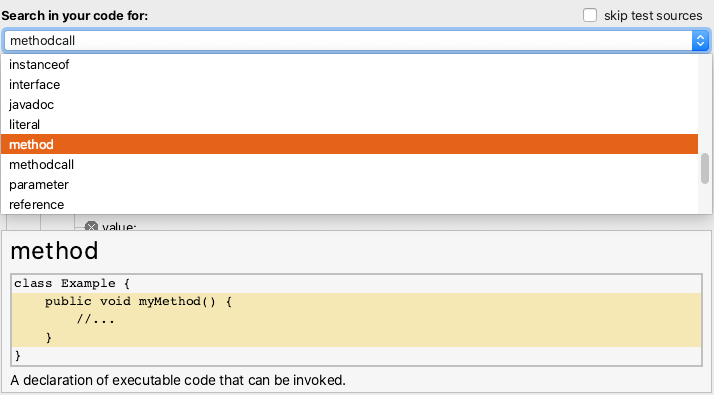
\includegraphics[width=\textwidth]{dropdownhint.png}
  \includegraphics[width=\textwidth,page=6]{04-tools/figures/figures1.pdf}
  \caption[Hints for different syntactic components in the recipe editor]{There are hints available that describe the different syntactic components that can be used in Sensei recipes. These hints are visible when hovering over the different options in the drop-down menu of the recipe editor.}
  \label{fig:dropdownhint} 
\end{figure}

In the fix menu it is possible to reuse arguments of the original code through a template language..
All users who made use of these templates, did so by copying the template from a different recipe and adjusting it to their needs.
None of the users used the suggestions available in the fix menu.

\subsection{Threats to validity}
There are many threats to the validity of conclusions drawn from the findings of these usability tests.
The number of subjects is small and the tasks they were asked to complete are artificial.
The focus of these tests is not to generalize any of the behaviours of the subjects, but rather to identify common usability problems in the interface of the recipe editor.
Several of these problems were detected.
I make no further attempts at interpreting the results from this usability test, I only report the findings as they appeared in the screen recordings.
\section{Industry trial in 2018}
\label{sec:trial2018}

One of the earliest customers of Sensei closely monitored their use of the tool during a trial period of several months in 2018.
They reported their findings to us and at the end of the trial they purchased additional licenses for the tool.

\subsection{Goal}
The \textit{goal} of the trial is for the client to observe the effects of the Sensei \gls{ide} plugin on its development process.
The \textit{purpose} is to help the client decide whether or not it is worth to purchase licenses for the Sensei \gls{ide} plugin.
The \textit{quality focus} is on the time and money saved by detecting possible vulnerabilities early.
The client aims at better estimating the return on investment of the potential purchase.
During the trial they can both collect some objective data on the amount of vulnerabilities prevented, as well as collect opinions from the application security team and the developers involved in the trial.

\subsection{Set-up}
\subsubsection{Subjects}
The client is a large bank included among the top 25 banks of the world as listed on wikipedia\footnote{\url{https://en.wikipedia.org/wiki/List\_of\_largest\_banks}}. The subjects were a group of five full-time developers selected by the client for their security knowledge. The tool was also given to an employee responsible for application security to help evaluate the trial. This employee was our main contact during the trial period.

\subsubsection{Tasks}
The subjects are part of teams developing and maintaining the web and mobile applications of the client. They were developing in either IntelliJ IDEA or Android Studio. During the trial period they continued their daily responsibilities as usual, reporting periodically to the application security expert on their impressions of the tool.

\subsubsection{Treatment}
The developers were given two sets of recipes, one for general Java applications, and one for mobile Android applications in particular.
The cookbook for general Java applications was developed internally by our developers in cooperation with the application security expert.
They advised what they wanted to achieve from the developers with the tool, and we created recipes to enforce this.
The second cookbook was also developed by us and was based on the official Android developer guidelines\footnote{\url{https://developer.android.com/}}.
All of the recipes in this set had scopes so they would only be active when the developer is working on an Android project.

\subsubsection{Information gathering}
The client did not share their code nor their Sensei events file.
Our contact was given the ability to view the summary of the Sensei events file in the form of an update to the Sensei plugin that enables them to view the statistics on each device.
Our contact at the company evaluated these and shared some of their insights as well as opinions from the subjects themselves.

\subsection{Findings}
They reported that during the trial over 200 markings were found that were legitimate markings that could lead to vulnerabilities. With the majority of these present in legacy code, they were \glspl{security defect} already in production. The two most common categories were mentioned as being tapjacking and sensitive information leakage (mostly caused by leaking stack traces).

The subjects reported the tool as very useful and not too intrusive when working on new code. They also reported improving their security knowledge, driven by the markings from the plugin.

After the trial, the client chose to extend their current licenses and purchase additional ones.

\subsection{Threats to validity}
There are many threats to the validity of conclusions drawn from the findings of this trial. We have no detailed knowledge or control over the task, the subjects, the time, or indeed over any other aspect of the trial. We are unable to account for any noise in the metrics or any conditions that limit our ability to generalize the results. For this reason we make no attempts at interpreting the results from this trial, we only report the findings as they were reported to us.
\section{Industry interview in 2021}
\label{sec:trial}

%Intro
%-------
%    Pieter - PhD in software security at SCW and University of Ghent Belgium
%    Research DevSecOps - human centered security practices
%    Some questions you might not have the answer available without looking up data
%    I will come back with an e-mail and we can see what data is possible 
%    Can I record this meeting? that way I don't have to take notes
%    Who are you? What are your roles at the company?
%    
%Team and practices
%------------------
%    How long have you been using Sensei? 
%    Size of the team? devs vs security professionals
%    How many use Sensei? Voluntarily? Changed over time?
%    How did you start using it?
%    What other tools do you use that work well or work against Sensei?
%    
%Rules creation
%--------------
%    How many Sensei rules have you created?
%    Who creates the rules?
%        - wizard? preview panels? UI view or code view?
%        - quickfixes? descriptions? scopes?
%        - do they have lots of hits?
%    Security related vs quality vs productivity?
%    Recipes to migrate libraries? Or recipes to use libraries correctly?
%    do you use any public cookbooks?
%    any rules that stand out to you, that you think show off Sensei capabilities?
%    
%Findings
%--------
%    do your rules have hits on code that you don't want to fix? or are they always accurate?
%    do the users of Sensei trust the tool and quickfixes? do they use them often?
%    Do you feel Sensei improces your code security? Do you have any evidence?
%    Do you feel Sensei boosts productivity?
%    
%    Overall impressions of Sensei?
%        - security, quality, productivity, management

In August 2021 I had the opportunity to interview the security team at a large company that has been using Sensei for over two years.
They shared their insights in how the tool is used, what they liked about it and what its biggest shortcomings are in their eyes. 
        
\subsection{Goal}
The \textit{goal} of this interview is to learn how Sensei is actually used in an industry setting.
The \textit{purpose} is to understand if our design goals align with the expectations of the users, and to observe which features are most useful and which are lacking or missing.
The \textit{quality focus} is on the frequency features are being used, and for which purpose.

\subsection{Set-up}

\subsubsection{Subjects}
The client is an international cloud computing company building and maintaining \gls{erp} software used by more than 26,000 customers.
The teams observed and interviewed are based in Europe.
They are 8 teams of developers and a team of 12 security professionals.
Most, but not all, security professionals have prior development experience, some at this same company.

\subsubsection{Task}
The subjects are part of teams developing and maintaining the \gls{erp} software of the client.
All of the Sensei users are developing using the IntelliJ IDEA.
During the use of Sensei they have continued their daily responsibilities as usual.

\subsubsection{Treatement}
Use of the Sensei plugin in these teams is voluntary.
About 90 employees in total are using the tool, of which 60 are using it more actively.
Five of the security professionals use the tool, as they are the ones involved in Java development.
The remaining users are developers.

The teams have been using Sensei for over two years.
When it was purchased, one of the security professionals gave a presentation and a demonstration of the tool to interested coworkers.
Most attendees were team leads, managers, and some security champions.
From there on, use of Sensei has not been actively promoted across the company.
However, one security professional regularly discusses the tool in the security champions group meetings, as well as the dedicated support channel on \gls{slack}.

The security team also uses Fortify, Checkmarx, SonarQube, Semgrep, and FindBugs.
They have sufficient context to compare Sensei to other security tools.
The listed tools, together with other comparable tools, are discussed in more detail in Chapter~\ref{ch:related}.

\subsubsection{Information gathering}
The team of security professionals is our contact at the company.
Two members of the team agreed to a meeting in which I interviewed them on their use and their impressions of Sensei as well as other security tools they are familiar with.
This interview was recorded and the recording reviewed before writing this report.

One of the interviewees has been with the company the entire time that Sensei was purchased, this person has prior development experience.
The other interviewee joined the company after the purchase of Sensei, this person does not have prior development experience, but has been a security professional for a longer time.

\subsection{Findings}

\subsubsection{Adoption}
The security professionals found that adoption of the tool is not easy.
It is hard to get a chance to show value to the developers, and they are hesitant to install new tools in their \gls{ide}.
It is easier to convince the security champions who are more interested, and actively looking for tools that can help them produce secure code faster.
So far the security professionals have preferred the hands-off approach and allowed the tool to organically spread, instead of making it mandatory.
The security professionals, many who have development backgrounds, are convinced that the tool can be an asset to developers outside of the context of security as well.

\subsubsection{Recipes}
The security professionals have created around 50 recipes.
They are stored on a remote server and distributed to the developers as a read-only cookbook.
The recipes in this cookbook are not all security related, but around 70\% of them are.
The other recipes are related to quality and code conventions.
Many of the security team have a development background, they have added these recipes in an attempt to show their value to the developers.
No public cookbooks are used, but the recipes in the public cookbooks served as inspiration for their own custom recipes.

The company has a lot of very clear coding standards that are published and used outside of their company as well.
These coding standards are used as a basis for recipes and their quick-fixes.
No real consultation with developers is needed, as it is generally agreed by developers and security experts that these coding standards are to be used.
However, to create the quick-fixes, the security professionals frequently consult internally with more experienced team members.
Since some of them are former developers at the same company, they have an intimate knowledge of the code base.

The company uses many wrapper libraries.
However, these are often not specifically written for security purposes only.
Several Sensei recipes exist to migrate to wrapper libraries or to different versions of \glspl{api}.

The security team is currently unaware of the amount of recipes that are being created by developers themselves.
They are also unaware if developers are frequently remediating markings from the distributed cookbook.
In fact, in their eyes, visibility into metrics like this is one of the biggest shortcomings of the tool.

\subsubsection{Recipe editor}
The security professionals create both recipes from scratch and from context and think both use cases are important and necessary.
They most frequently use the \gls{ui} view to edit recipes, but to refactor recipes and make bulk changes, they sometimes use a text editor as well.

They think the preview panels and the recipe editor are by far the most useful features of the entire plugin.
These features make customization of the recipes far more easy compared to the other tools they are using in the \gls{sdlc}.

Descriptions are often used, but the full coding guidelines are not usually customized to the specific recipe.
The coding guideline provided is instead a generally applicable description that provides links to documentation about the secure coding standards that are used at the company.

The security professionals use recipe scopes very often.
The scopes are used to limit recipes to certain packages and modules.
This is only done as a consideration for developer usability, to avoid false positives in the large code base.

Finally, they try to provide quick-fixes as often as possible, but admit it is not always possible.
Sometimes the quick-fix provided requires the developer to make additional changes.

\subsubsection{Paved path methodology}
The security team is not using a paved path methodology.
However, their practices are in line with many of the goals of this methodology.

The security professionals try to be \textit{enablers}, and not only tell developers what they do wrong, but also provide guidance as much as possible.
They provide a service to developers and are very aware of developer usability.
The team prefers to neglect some parts of the security of the software over generating too many false positives, which could result in \glspl{efp}.

They belief Sensei supports this enablement approach through its quick-fixes.
Since a complete Sensei recipe includes a quick-fix, the security team is forced to offer remediation guidance.
This remediation guidance in turn enables the developers to resolve security markings by themselves.

For the security professionals without former development experience, this requirement of a quick-fix forces them to be closer to the development workflows.
Sometimes, creating a quick-fix pushes the limits of their knowledge of programming.
In that case, they do not consult the development team, as suggested by the paved path methodology, but instead consult with former developers in the security team itself.

\subsubsection{Disadvantages}
As mentioned before, visibility into the developer's practices with the tool is one of the biggest shortcomings of Sensei in the eyes of the security team.
So far features that report back information from the \gls{ide} have been avoided as we expected customers would be hesitant of such features.
Many of the metrics that the security team requests are available in the \glspl{ide} of the developers, in the Sensei events databases.
Clearly, gathering those databases is not a convenient way to collect that information.
On top of that, currently we provide no convenient way visualize the results in a management dashboard, which other tools commonly provide.

Alternatively, some metrics can be collected through server side scans.
It is possible to run IntelliJ IDEA inspections from the command line, including the Sensei recipes. 
The resulting scans are not as efficient as those by standalone tools, such as static analysis tools discussed in Chapter~\ref{ch:related}.
In particular, the memory usage is exceedingly big for large enough code bases because the entire \gls{ide} is in fact running in a background process.
It is also more difficulty to automate running IntelliJ IDEA inspections in the \gls{cicd} pipeline compared to tools who provide better integrations for this purpose.
The convenience of running scans in other stages of the \gls{sdlc} seems to be the main reason the security team uses some of the other tools.

%
%== Other tools
%FindBugs
%--------
%Creating rules with is harder, not as intuitive
%Can be more easily integrated in CI
%Simple general rules that are more widely applicable, and make more sense in CI
%Not usable in shift left
%No remediation
%They want rules in CI and in the IDE to show the same things
%
%SemGrep
%-------
%used by security professionals in the code reviews, in between developing and building
%without dev, reactive feedback, more automated
%links to documentation as feedback, no code fixes
%rules are pretty easy to customize but it is more difficult without the preview panels, it is better than findbugs
%semgrep is multi language
%compile agnostic, fully realised on text (no AST), so no compilable classes are required, code snippets are enough
%
\subsection{Threats to validity}
There are many threats to the validity of conclusions drawn from the findings of this trial. We have no detailed knowledge or control over the task, the subjects, the time, or indeed over any other aspect of the trial. We are unable to account for any noise in the metrics or any conditions that limit our ability to generalize the results. For this reason we make no attempts at interpreting the results from this trial, we only report the findings as they were reported to us.
%\section{Marketplace users}
\label{sec:marketplace}

The Sensei \gls{ide} plugin has been release for free on the JetBrains marketplace on September 10, 2020.
During this time many developers have installed and uninstalled the plugin.
We have collected metrics to give us insights into what makes a user keep using Sensei, or what causes them to uninstall it.


%Churn rate:
%(confidential? Can I share this data? Probably not)
%the insights might be useful, but the exact numbers can not be shared
%
%Opened cookbook manager:
%never, 350, 134
%once, 64, 61
%twice, 24, 26
%3 or more times, 34, 67
%
%Added cookbooks in the cookbook manager
%0 cookbooks, 109, 141
%1 cookbooks, 13, 13
%
%Churn by days till the cookbook manager is opened
%never opened, 490, 154
%day 0, 123, 103
%day 1, 7, 9
%day 2+, 24, 87
%
%churn by opening recipe editor
%0 times, 456, 258
%1+, 15, 21
%
%churn by days till open recipe editor
%never opened, 624, 318
%0-1 day, 16, 11
%1+ days, 5, 26
%
%Most people install early on:
%Most people who make it past a week, stick around 

